% Options for packages loaded elsewhere
\PassOptionsToPackage{unicode}{hyperref}
\PassOptionsToPackage{hyphens}{url}
%
\documentclass[
  man, donotrepeattitle,floatsintext]{apa6}
\usepackage{amsmath,amssymb}
\usepackage{lmodern}
\usepackage{iftex}
\ifPDFTeX
  \usepackage[T1]{fontenc}
  \usepackage[utf8]{inputenc}
  \usepackage{textcomp} % provide euro and other symbols
\else % if luatex or xetex
  \usepackage{unicode-math}
  \defaultfontfeatures{Scale=MatchLowercase}
  \defaultfontfeatures[\rmfamily]{Ligatures=TeX,Scale=1}
\fi
% Use upquote if available, for straight quotes in verbatim environments
\IfFileExists{upquote.sty}{\usepackage{upquote}}{}
\IfFileExists{microtype.sty}{% use microtype if available
  \usepackage[]{microtype}
  \UseMicrotypeSet[protrusion]{basicmath} % disable protrusion for tt fonts
}{}
\makeatletter
\@ifundefined{KOMAClassName}{% if non-KOMA class
  \IfFileExists{parskip.sty}{%
    \usepackage{parskip}
  }{% else
    \setlength{\parindent}{0pt}
    \setlength{\parskip}{6pt plus 2pt minus 1pt}}
}{% if KOMA class
  \KOMAoptions{parskip=half}}
\makeatother
\usepackage{xcolor}
\usepackage{graphicx}
\makeatletter
\def\maxwidth{\ifdim\Gin@nat@width>\linewidth\linewidth\else\Gin@nat@width\fi}
\def\maxheight{\ifdim\Gin@nat@height>\textheight\textheight\else\Gin@nat@height\fi}
\makeatother
% Scale images if necessary, so that they will not overflow the page
% margins by default, and it is still possible to overwrite the defaults
% using explicit options in \includegraphics[width, height, ...]{}
\setkeys{Gin}{width=\maxwidth,height=\maxheight,keepaspectratio}
% Set default figure placement to htbp
\makeatletter
\def\fps@figure{htbp}
\makeatother
\setlength{\emergencystretch}{3em} % prevent overfull lines
\providecommand{\tightlist}{%
  \setlength{\itemsep}{0pt}\setlength{\parskip}{0pt}}
\setcounter{secnumdepth}{-\maxdimen} % remove section numbering
% Make \paragraph and \subparagraph free-standing
\ifx\paragraph\undefined\else
  \let\oldparagraph\paragraph
  \renewcommand{\paragraph}[1]{\oldparagraph{#1}\mbox{}}
\fi
\ifx\subparagraph\undefined\else
  \let\oldsubparagraph\subparagraph
  \renewcommand{\subparagraph}[1]{\oldsubparagraph{#1}\mbox{}}
\fi
\newlength{\cslhangindent}
\setlength{\cslhangindent}{1.5em}
\newlength{\csllabelwidth}
\setlength{\csllabelwidth}{3em}
\newlength{\cslentryspacingunit} % times entry-spacing
\setlength{\cslentryspacingunit}{\parskip}
\newenvironment{CSLReferences}[2] % #1 hanging-ident, #2 entry spacing
 {% don't indent paragraphs
  \setlength{\parindent}{0pt}
  % turn on hanging indent if param 1 is 1
  \ifodd #1
  \let\oldpar\par
  \def\par{\hangindent=\cslhangindent\oldpar}
  \fi
  % set entry spacing
  \setlength{\parskip}{#2\cslentryspacingunit}
 }%
 {}
\usepackage{calc}
\newcommand{\CSLBlock}[1]{#1\hfill\break}
\newcommand{\CSLLeftMargin}[1]{\parbox[t]{\csllabelwidth}{#1}}
\newcommand{\CSLRightInline}[1]{\parbox[t]{\linewidth - \csllabelwidth}{#1}\break}
\newcommand{\CSLIndent}[1]{\hspace{\cslhangindent}#1}
\ifLuaTeX
\usepackage[bidi=basic]{babel}
\else
\usepackage[bidi=default]{babel}
\fi
\babelprovide[main,import]{english}
% get rid of language-specific shorthands (see #6817):
\let\LanguageShortHands\languageshorthands
\def\languageshorthands#1{}
% Manuscript styling
\usepackage{upgreek}
\captionsetup{font=singlespacing,justification=justified}

% Table formatting
\usepackage{longtable}
\usepackage{lscape}
% \usepackage[counterclockwise]{rotating}   % Landscape page setup for large tables
\usepackage{multirow}		% Table styling
\usepackage{tabularx}		% Control Column width
\usepackage[flushleft]{threeparttable}	% Allows for three part tables with a specified notes section
\usepackage{threeparttablex}            % Lets threeparttable work with longtable

% Create new environments so endfloat can handle them
% \newenvironment{ltable}
%   {\begin{landscape}\centering\begin{threeparttable}}
%   {\end{threeparttable}\end{landscape}}
\newenvironment{lltable}{\begin{landscape}\centering\begin{ThreePartTable}}{\end{ThreePartTable}\end{landscape}}

% Enables adjusting longtable caption width to table width
% Solution found at http://golatex.de/longtable-mit-caption-so-breit-wie-die-tabelle-t15767.html
\makeatletter
\newcommand\LastLTentrywidth{1em}
\newlength\longtablewidth
\setlength{\longtablewidth}{1in}
\newcommand{\getlongtablewidth}{\begingroup \ifcsname LT@\roman{LT@tables}\endcsname \global\longtablewidth=0pt \renewcommand{\LT@entry}[2]{\global\advance\longtablewidth by ##2\relax\gdef\LastLTentrywidth{##2}}\@nameuse{LT@\roman{LT@tables}} \fi \endgroup}

% \setlength{\parindent}{0.5in}
% \setlength{\parskip}{0pt plus 0pt minus 0pt}

% Overwrite redefinition of paragraph and subparagraph by the default LaTeX template
% See https://github.com/crsh/papaja/issues/292
\makeatletter
\renewcommand{\paragraph}{\@startsection{paragraph}{4}{\parindent}%
  {0\baselineskip \@plus 0.2ex \@minus 0.2ex}%
  {-1em}%
  {\normalfont\normalsize\bfseries\itshape\typesectitle}}

\renewcommand{\subparagraph}[1]{\@startsection{subparagraph}{5}{1em}%
  {0\baselineskip \@plus 0.2ex \@minus 0.2ex}%
  {-\z@\relax}%
  {\normalfont\normalsize\itshape\hspace{\parindent}{#1}\textit{\addperi}}{\relax}}
\makeatother

% \usepackage{etoolbox}
\makeatletter
\patchcmd{\HyOrg@maketitle}
  {\section{\normalfont\normalsize\abstractname}}
  {\section*{\normalfont\normalsize\abstractname}}
  {}{\typeout{Failed to patch abstract.}}
\patchcmd{\HyOrg@maketitle}
  {\section{\protect\normalfont{\@title}}}
  {\section*{\protect\normalfont{\@title}}}
  {}{\typeout{Failed to patch title.}}
\makeatother

\usepackage{xpatch}
\makeatletter
\xapptocmd\appendix
  {\xapptocmd\section
    {\addcontentsline{toc}{section}{\appendixname\ifoneappendix\else~\theappendix\fi\\: #1}}
    {}{\InnerPatchFailed}%
  }
{}{\PatchFailed}
\DeclareDelayedFloatFlavor{ThreePartTable}{table}
\DeclareDelayedFloatFlavor{lltable}{table}
\DeclareDelayedFloatFlavor*{longtable}{table}
\makeatletter
\renewcommand{\efloat@iwrite}[1]{\immediate\expandafter\protected@write\csname efloat@post#1\endcsname{}}
\makeatother
\usepackage{lineno}

\linenumbers
\usepackage{csquotes}
\ifLuaTeX
  \usepackage{selnolig}  % disable illegal ligatures
\fi
\IfFileExists{bookmark.sty}{\usepackage{bookmark}}{\usepackage{hyperref}}
\IfFileExists{xurl.sty}{\usepackage{xurl}}{} % add URL line breaks if available
\urlstyle{same} % disable monospaced font for URLs
\hypersetup{
  pdftitle={Manybabies1 Test-Retest Supplementary Information},
  pdflang={en-EN},
  hidelinks,
  pdfcreator={LaTeX via pandoc}}

\title{Manybabies1 Test-Retest Supplementary Information}
\author{\phantom{0}}
\date{}


\shorttitle{MB1T supplementary}

\affiliation{\phantom{0}}

\begin{document}
\maketitle

\hypertarget{s1-relationship-between-the-number-of-trials-infants-contribute-in-each-session}{%
\subsection{S1: Relationship between the number of trials infants contribute in each session}\label{s1-relationship-between-the-number-of-trials-infants-contribute-in-each-session}}

\begin{figure}
\centering
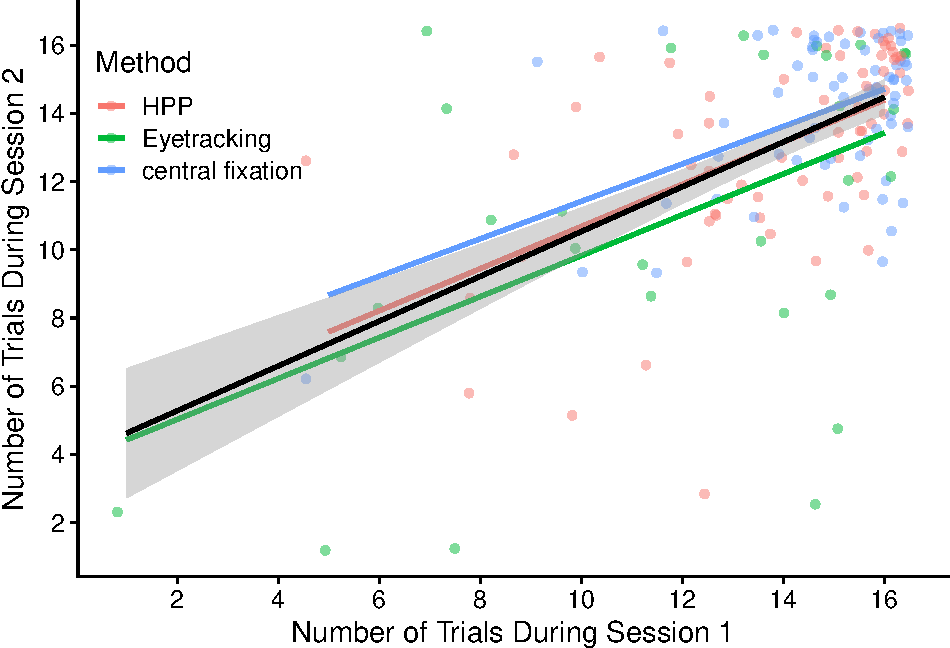
\includegraphics{MB1T_supplement_files/figure-latex/sfig1-1.pdf}
\caption{\label{fig:sfig1}Correlation between the number of trials contributed in session 1 and session 2. Each data point represents one infant. Colored lines represent linear fits for each method.}
\end{figure}

Are there stable individual differences in how likely an infant is to contribute a high number of trials?
To answer this question, we conducted an exploratory analysis investigating whether there is a relationship between the number of trials an infant contributed in session 1 and session 2.
Do infants who contribute a higher number of trials during their first testing session also tend to contribute more trials during their second testing session?
A positive correlation between trial numbers during the first and second session would indicate that their is some stability in a given infants' likelihood of remaining attentive throughout the experiment.
On the other hand, the absence of a correlation would indicate that the number of trials a given infant contributes is not predictive of how many trials they might contribute during their next session.

We found a strong positive correlation between number of trials contributed during the first and the second session \(r = .58\), 95\% CI \([.47, .68]\), \(t(159) = 9.05\), \(p < .001\) (see Figure 1).
This result suggests that if infants contribute a higher number of trials in one session, compared to other infants, they are likely to contribute a higher number of trials in their next session.
This finding is consistent with the hypothesis that how attentive infants are throughout an experiment (and hence how many trials they contribute) is a stable individual difference, at least for some infant looking time tasks.
Researchers should therefore be mindful of the fact that decisions about including or excluding infants based on trials contributed may selectively sample a specific sub-set of the infant population they are studying (Byers-Heinlein, Bergmann, \& Savalei, 2021; DeBolt, Rhemtulla, \& Oakes, 2020).

\hypertarget{s2-preference-reversal}{%
\subsection{S2: Preference reversal}\label{s2-preference-reversal}}

48.48 percent of the infants had a preference reversal from test to retest session.

\hypertarget{s3-deviations-from-the-preregistration}{%
\subsection{S3: Deviations from the preregistration}\label{s3-deviations-from-the-preregistration}}

Below, we document all deviations from the preregistered methods and analyses \url{https://osf.io/v5f8t}.

\begin{itemize}
\tightlist
\item
  All infants with usable data for both test and retest session were included in the analyses, regardless of the number of total of infants a lab was able to contribute after exclusion. This decision is consistent with past decisions in ManyBabies projects to be as inclusive about data inclusion as possible (ManyBabies Consortium, 2020).
\item
  A small number of infants with a time between sessions above 31 days were also included in the analyses (n=2).
\item
  Consistent with analytic decisions in ManyBabies 1 (ManyBabies Consortium, 2020), total looking times were truncated at 18 seconds (the maximum trial time) in the small number of cases where recorded looking times were slightly greater than 18s (presumably due to small measurement error in recording infant looking times).
\end{itemize}

\newpage

\hypertarget{references}{%
\section{References}\label{references}}

\begingroup
\setlength{\parindent}{-0.5in}
\setlength{\leftskip}{0.5in}

\hypertarget{refs}{}
\begin{CSLReferences}{1}{0}
\leavevmode\vadjust pre{\hypertarget{ref-byers2021six}{}}%
Byers-Heinlein, K., Bergmann, C., \& Savalei, V. (2021). Six solutions for more reliable infant research. \emph{Infant and Child Development}, e2296.

\leavevmode\vadjust pre{\hypertarget{ref-debolt2020robust}{}}%
DeBolt, M. C., Rhemtulla, M., \& Oakes, L. M. (2020). Robust data and power in infant research: A case study of the effect of number of infants and number of trials in visual preference procedures. \emph{Infancy}, \emph{25}(4), 393--419.

\leavevmode\vadjust pre{\hypertarget{ref-manybabies2020quantifying}{}}%
ManyBabies Consortium. (2020). Quantifying sources of variability in infancy research using the infant-directed-speech preference. \emph{Advances in Methods and Practices in Psychological Science}, \emph{3}(1), 24--52.

\end{CSLReferences}

\endgroup


\end{document}
